\documentclass[../main/main.tex]{subfiles}
\graphicspath{{./figures/}}

\makeatletter
\renewcommand{\@chapapp}{Travaux pratiques -- TP}
\makeatother

\toggletrue{student}
\HideSolutionstrue

\begin{document}
\setcounter{chapter}{6}

\chapter{Circuits du premier ordre en r\'egime transitoire}

\ifstudent{
	\begin{prgm}
		\begin{tcb}*(ror)"know"{Savoirs}
			\begin{itemize}[label=$\diamond$, leftmargin=10pt]
				\item Distinguer, sur un relevé expérimental, régime
				      transitoire et régime permanent au cours de l'évolution d'un
				      système du premier ordre soumis à un échelon de tension.
			\end{itemize}
		\end{tcb}
		\begin{tcb}*(ror)"how"{Savoir-faire}
			\begin{itemize}[label=$\diamond$, leftmargin=10pt]
				\item Réaliser l'acquisition d'un régime transitoire pour un circuit
				      linéaire du premier ordre et analyser ses caractéristiques.
				      Confronter les résultats expérimentaux aux expressions théoriques.
				\item Capacité numérique : mettre en œuvre la méthode
				      d'\textsc{Euler} à l'aide d'un langage de programmation pour
				      simuler la réponse d'un système linéaire du premier ordre à une
				      excitation de forme quelconque.
			\end{itemize}
		\end{tcb}
	\end{prgm}
	\vspace{-10pt}
	\section{Objectifs}
	\begin{itemize}
		\item Réaliser des montages simples d'électricité.
		\item Déterminer expérimentalement un temps de relaxation.
		\item Observer les différents paramètres qui influent sur un régime
		      transitoire.
		\item Observer les différents régimes du second ordre.
		\item Découvrir quelques fonctions nouvelles de l'oscilloscope et du GBF.
		\item Mettre en œuvre la méthode d'\textsc{Euler} à l'aide de Python pour
		      simuler la réponse d'un système linéaire du premier ordre à une
		      excitation
		      quelconque.
	\end{itemize}
}

\section{S'approprier}

\begin{tcb}(rapp){Règles de bonne pratique}
	\begin{itemize}
		\item En pratique, on commence toujours par effectuer les branchements du
		      circuit sans insérer les appareils de mesure.
		\item Puis, on \textbf{relie toutes les masses entre elles} afin d'éviter de
		      fixer par erreur une autre masse dans le circuit. Ainsi, un bon circuit
		      aura une «~ligne de masse~» à laquelle seront reliés obligatoirement tous
		      les câbles noirs provenant des câbles coaxiaux-filaires reliés à
		      l'oscilloscope ou au GBF.
		\item Enfin, on place alors les fils colorés des câbles de mesure aux
		      endroits où on désire relever la tension. Vous serez d'ailleurs
		      également vigilant au choix de couleurs des fils, sinon on se perd
		      rapidement…
	\end{itemize}
	Ces règles sont fondamentales et ne doivent pas être négligées si
	on veut que le circuit fonctionne.
\end{tcb}

\subsection{Circuit intégrateur}

Un montage est considéré comme \textbf{intégrateur} (on le verra en cours dans
quelques semaines) si la tension de sortie (dans notre cas $u_{c}(t)$) est une
primitive, à une constante multiplicative $K$ près, de la tension d'entrée (dans
notre cas $e(t)$), soit encore

\[u_{c}(t) = K \int e(t) \dt\]

\subsection{Détermination numérique de la solution}
\subsubsection{Position du problème}

Soit $u_{C}(t)$ est solution de l'équation différentielle~:
\[
	\dv{u_C(t)}{t} + \frac{u_C(t)}{\tau} = \frac{e(t)}{\tau}
\]

L'objectif de cette partie est de déterminer \textbf{numériquement} la solution
$u_{C}(t)$ de cette équation pour une entrée quelconque $e(t)$ pour laquelle il
n'existe pas toujours de solutions analytiques. Nous allons utiliser un schéma
numérique classique appelé Méthode d'\textsc{Euler}.

En pratique, cette méthode est relativement peu efficace (et des méthodes plus
sophistiquées sont souvent mises en place). Néanmoins la méthode
d'\textsc{Euler}, très simple à comprendre et à mettre en place, permet une
première approche simple du problème.

\subsubsection{Méthode d'\textsc{Euler}~: mathématiquement}
\label{sssec:euler}

Des théorèmes assurent que, sous des conditions raisonnables, il existe une
unique application $y$ de classe $C^1$ sur $[a,b]$ dont la valeur est imposée en
$a$ et qui vérifie une équation différentielle de la forme $y'(t)=f(t,y(t))$
pour tout $t \in [a,b]$. L'objet des \textit{schémas numériques} est d'obtenir
des approximations de cette solution.
\bigbreak
\noindent
\begin{minipage}[c]{.55\linewidth}
	En pratique, on tente d'approcher $y$ en un certain nombre de points répartis
	sur l'intervalle $[a,b]$. Plus précisément, on veut calculer une approximation
	$y_k$ des $y(t_k)$ avec $t_k=a+kh$ où $h=\dfrac{b-a}{n}$ est un pas qu'il
	conviendra d'ajuster (on peut supposer que plus le pas est petit, meilleure sera
	l'approximation). De façon simple, on peut écrire~:
	\begin{align*}
		y(t_{k+1})-y(t_k) & =
		\int_{t_k}^{t_{k+1}}y'(u) \dd u =
		\int_{t_k}^{t_{k+1}} f(u,y(u)) \dd u
		\\\Lra
		y(t_{k+1})-y(t_k) & \approx h f(t_k,y(t_k))
	\end{align*}
\end{minipage}
\hfill
\begin{minipage}[c]{.45\linewidth}
	~
	\begin{center}
		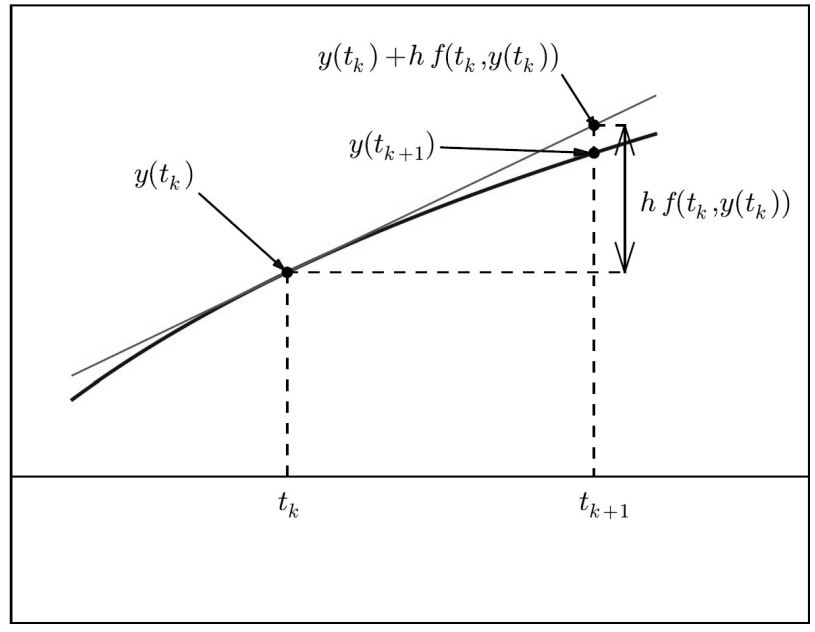
\includegraphics[width=\linewidth]{euler}
	\end{center}
\end{minipage}
\bigbreak
On obtient alors la méthode d'\textsc{Euler} explicite~: les approximations sont
calculées de proche en proche via la formule suivante~:
\[\boxed{y_{k+1}=y_k+hf(t_k,y_k)}\]
On initialise bien entendu avec $y_0=y(a)$, qui sera la seule valeur «~exacte~»
calculée.

\section{Analyser : régime transitoire du circuit RC}

\begin{tcb}[cnt, bld](impo){}
	Vous prendrez soin de refaire tous les schémas des circuits mis en place ou
	étudiés.
\end{tcb}
\begin{tcb}*(prop)"bomb"{Attention}
	Pour ce TP, il vous est demandé de rédiger les réponses préalables sur vos
	comptes-rendus, \textbf{en amont} du TP.
\end{tcb}

\subsection{Charge et décharge du condensateur}
\label{ssec:chdech}

On considère le montage ci-contre de constante de temps $\tau = RC$.

\noindent
\begin{minipage}[t]{.65\linewidth}
	\begin{enumerate}[label=\clenumi]
		\item Si $e(t)$ est une tension créneau de fréquence $f = \SI{1}{kHz}$,
		      quelle valeur faut-il donner à $\tau$ pour visualiser de façon
		      satisfaisante la totalité du régime transitoire~? Expliquer les raisons
		      de votre choix.
		\item Si $\tau$ est trop grand ou si $\tau$ est trop petit, que se
		      passe-t-il~?
	\end{enumerate}
\end{minipage}
\hfill
\begin{minipage}[t]{.30\linewidth}
	~
	\begin{center}
		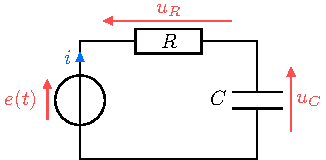
\includegraphics[width=\linewidth]{circ_rc-start}
	\end{center}
\end{minipage}

\begin{enumerate}[label=\clenumi, start=3]
	\item Si $R = \SI{1}{k\Omega}$, quelle valeur faut-il alors donner à $C$~?
	\item On veut visualiser à l'oscilloscope simultanément $e(t)$ sur la voie 1
	      et $u_{C}(t)$ sur la voie 2~; indiquer sur un schéma les connexions à
	      réaliser.
\end{enumerate}

\subsection{Étude théorique du circuit intégrateur}
\label{ssec:cint}

L'équation différentielle vérifiée par $u_{C}(t)$ est

\[\frac{\dd u_{C}(t)}{\dd t} + \frac{u_{C}(t)}{\tau} = \frac{e(t)}{\tau}\]

Supposons que à $t=0$, $e(t)$ passe de $0$ à $E$.

\begin{enumerate}[label=\clenumi, resume]
  \item \label{q:sol}
        Déterminer la solution de l'équation différentielle précédente dans
	      le cas où $u_{C}(t=0) = 0$. En utilisant un développement limité du
	      terme exponentiel autour de $t = 0$, montrer que le montage est
	      intégrateur (la sortie est une primitive de l'entrée).
\end{enumerate}

\medskip

\begin{tcb}*[aide](expe)<itc>{Aide}
	Le développement limité de l'exponentiel s'écrit
	\[\text{e}^x \Sim_{x \to 0} 1+x + o(x)\]
\end{tcb}

\subsection{Circuit RC avec visualisation de $e(t)$ et $u_{R}(t)$}
\label{ssec:uR}

On souhaite maintenant visualiser $e(t)$ sur la voie 1 et $u_{R}(t)$ sur la voie
2.

\begin{enumerate}[label=\clenumi, resume]
	\item Comment faut-il modifier le montage~? Sur votre feuille, faire le
	      schéma du montage correspondant en indiquant les branchements de
	      l'oscilloscope.
	\item Écrire l'équation différentielle vérifiée par la variable $u_{R}(t)$
	      et en donner la solution pour $e(t) = E$ et $u_{R}(t=0^-) = 0$.
	      Attention, la tension n'est \textit{a priori} pas continue aux bornes de
	      $R$…
\end{enumerate}
\section{Réaliser et valider}
\subsection{Étude expérimentale du régime transitoire du circuit RC}

\subsubsection{Cas général~: charge et décharge du condensateur}

\begin{tcb}(expe){}
	\begin{enumerate}
		\item Réaliser le montage RC proposé dans la partie~III.A.
		\item $e(t)$ est une tension créneau (alternance de tension nulle et de
		      tension constante $E$) d'un générateur basses fréquences, réglé sur une
		      fréquence de $\SI{1}{kHz}$.
		\item $R$ est une boîte de résistances variables~; prendre $R =
			      \SI{1}{k\Omega}$.
		\item $C$ est une boîte de capacités réglables~; prendre la valeur calculée
		      dans la partir analyse.
		\item Observer $e(t)$ et $u_{C}(t)$.
		\item Imprimer vos courbes en suivant le protocole imprimé et plastifié sur
		      vos paillasses. \textbf{Pensez à inverser la couleur de l'écran pour
			      le pas imprimer sur un fond noir}.
	\end{enumerate}
\end{tcb}

\begin{enumerate}[label=\sqenumi]
	\item Déterminer la constante de temps $\tau_{\rm exp}$ ainsi que son
	      incertitude. Expliquer votre démarche.
	\item Calculer \textbf{et commenter} l'écart normalisé $E_N$ avec la valeur
	      théorique.
	\item Étudier l'influence de $R$ et de $C$. Faire varier également la
	      fréquence du signal périodique. Commenter vos observations. Il n'est pas
	      demandé de refaire de nouvelles mesures. Une analyse qualitative est
	      suffisante.
\end{enumerate}

\subsubsection{Cas particulier du circuit intégrateur}

\begin{tcb}*[cnt, bld](prop)"bomb"{Attention}
	Pour toute mesure, vérifier que la source du menu mesure correspond bien à
	la courbe sur laquelle vous faites des mesures.
\end{tcb}

\begin{enumerate}
	\item Ne pas modifier le montage précédent, $e(t)$ est toujours une tension
	      créneau. Choisir $\tau$ de l'ordre de $10 T$ en ajustant la valeur de
	      $R$ et observer $e(t)$ et $u_{C}(t)$.
	      \begin{enumerate}[label=\sqenumi, start=4]
		      \item Quelle est l'allure de $u_{C}(t)$~? $u_{C}(t)$ est-elle bien la
		            primitive de $e(t)$ à une constante multiplicative près?
		      \item Déterminer expérimentalement la pente de la courbe $u_{C}(t)$ en
		            vous aidant des curseurs. Comparer à la valeur théorique.
	      \end{enumerate}
	\item Conserver les valeurs de $\tau$ et $T$. Changer la tension créneau par
	      une dent de scie.
	      \begin{enumerate}[label=\sqenumi, start=6]
		      \item Quelle est l'allure de $u_{C}(t)$~? Le circuit est-il à priori
		            toujours intégrateur~?
		      \item Quelle est l'expression mathématique (aucun calcul à effectuer)
		            de la courbe $u_{C}(t)$~?
	      \end{enumerate}
	\item Conserver les valeurs de $\tau$ et $T$. Changer la tension créneau par
	      une tension sinusoïdale.
	      \begin{enumerate}[label=\sqenumi, start=8]
		      \item Quelle est l'allure de $u_{C}(t)$~? Le circuit est-il toujours
		            intégrateur~?
		      \item Quelle est l'expression mathématique (aucun calcul à effectuer)
		            de la courbe $u_{C}(t)$~?
	      \end{enumerate}
	\item Augmenter $\tau$.
	      \begin{enumerate}[label=\sqenumi, start=10]
		      \item Quel inconvénient apparaît~? Commenter vos observations.
	      \end{enumerate}
\end{enumerate}

\subsubsection{Tension aux bornes de la résistance $u_R$}

Se placer dans les mêmes conditions que dans la partie IV.A.1 et observer à
l'oscilloscope $e(t)$ et $u_{R}(t)$.
\begin{enumerate}[label=\sqenumi, start=11]
	\item Imprimer les résultats. Commenter l'allure
	      de la courbe. Est-elle conforme à l'expression analytique attendue~?
\end{enumerate}

\subsection{Étude numérique}
Effectuez cette étude sur \texttt{Capytale}~:
\url{https://capytale2.ac-paris.fr/web/c/bc8f-2174341}.

\subsubsection{Écriture du script}

% Vous avez dans un premier temps besoin d'importer les bibliothèques Python
% suivantes~:
%
% \begin{python}
% import matplotlib.pyplot as plt
% import numpy as np
% \end{python}

On créé la fonction \texttt{euler(f, a, b, y0, n)} effectuant les calculs
détaillés dans la partie~\ref{sssec:euler}. Ses paramètres d'entrée sont
une fonction $f$, des valeurs de $a$ et $b$, un entier $n$ et une
condition initiale $y0$. Elle calcule les valeurs approchées sur $[a,b]$ de la
solution de l'équation différentielle $y'(t)=f(t,y(t))$ avec la condition
initiale $y(a)=y0$. Cette fonction renvoie la liste des $n+1$ valeurs
approchées $y_k$ de $y$ aux temps $t_k=a+k \frac{b-a}{n}$, $k\in[\![0,n]\!]$.

% Compléter ensuite la fonction \texttt{euler(f, a, b, y0, n)} suivante qui, étant
% donnée une fonction $f$, des valeurs de $a$ et $b$, un entier $n$ et une
% condition initiale $y0$, calcule les valeurs approchées sur $[a,b]$ de la
% solution de l'équation différentielle $y'(t)=f(t,y(t))$ avec la condition
% initiale $y(a)=y0$. Cette fonction renverra la liste des $n+1$ valeurs
% approchées $y_k$ de $y$ aux temps $t_k=a+k \frac{b-a}{n}$, $k\in[\![0,n]\!]$.

\begin{python}
def euler(f, a, b, y0, n):
  h = (b-a) / n
  list_y = [y0]
  yk = y0
  tk = a
  for i in range(n):
    yk = # à compléter
    tk = # à compléter
    list_y.append(y)
  return list_y
\end{python}

Il faut ensuite créer la fonction \texttt{f} ainsi que la fonction entrée
\texttt{e} pour plus de clarté. Vous compléterez la fonction \texttt{f} pour
qu'elle renvoie l'expression correspondant à l'équation différentielle que vous
cherchez à résoudre.

% \begin{python}
% def f(t, y, e):
%   return # à compléter
%
% def e(t):
%   return 10 # à modifier, par exemple np.sin(t)
% \end{python}
%
% L'exemple proposé ici est dans le cas d'une entrée constante d'amplitude $E =
% 	10$. Vous pouvez alors changer la fonction \texttt{e(t)} si vous voulez explorer
% les solutions pour d'autres formes d'entrée.

On récupére les valeurs $y$ de la solution par~:
% tau = 1 # s
% list_t = np.linspace(0, 10, n+1) # vecteur temps entre t = 0 et t = 10 s
\begin{python}
list_y = euler(f, 0 , 10, 0, n) # list_y est un vecteur des valeurs de y
\end{python}

\subsubsection{Test dans un cas analytique}

Tester votre fonction précédente avec une entrée constante $e(t) = E$ afin de
résoudre l'équation différentielle sur $u_{C}(t)$. Afficher sur un même
graphique la solution numérique et la solution analytique obtenue
question~\ref{q:sol} (avant développement limité). On pourra, par choix et pour
fixer les idées, sans que cela porte à conséquence prendre~:

\[
  E = \SI{1}{V}
  \qquad \qquad
  \tau = \SI{1}{s}
  \qquad \qquad
  u_{C}(t=0) = 0
\]

Vous afficherez également la fonction erreur au cours du temps, qui est la
différence entre votre solution numérique et la solution analytique.
\begin{enumerate}[label=\sqenumi, start=12]
  \item Quelle est la sensibilité au pas de calcul~? Vous ferez plusieurs
    essais.
\end{enumerate}


\subsubsection{Test dans un cas non analytique}

Lorsque la solution $u_{C}(t)$ peut être obtenue analytiquement, la solution
numérique n'a que peu d'intérêt. Elle prend en revanche tout son sens dans des
cas non-analytiques.
\smallbreak
Testez votre programme pour plusieurs entrées (en changeant le contenu de la
fonction \texttt{e(t)})~: sinusoïdale, rampe linéaire, exponentielle…

\end{document}
